\section{Solving equations}
\begin{definition}
The function $f(x)$ has a \textbf{root} at $x = r$ if $f(r) = 0$.
\end{definition}

\subsubsection{The Bisection Method}
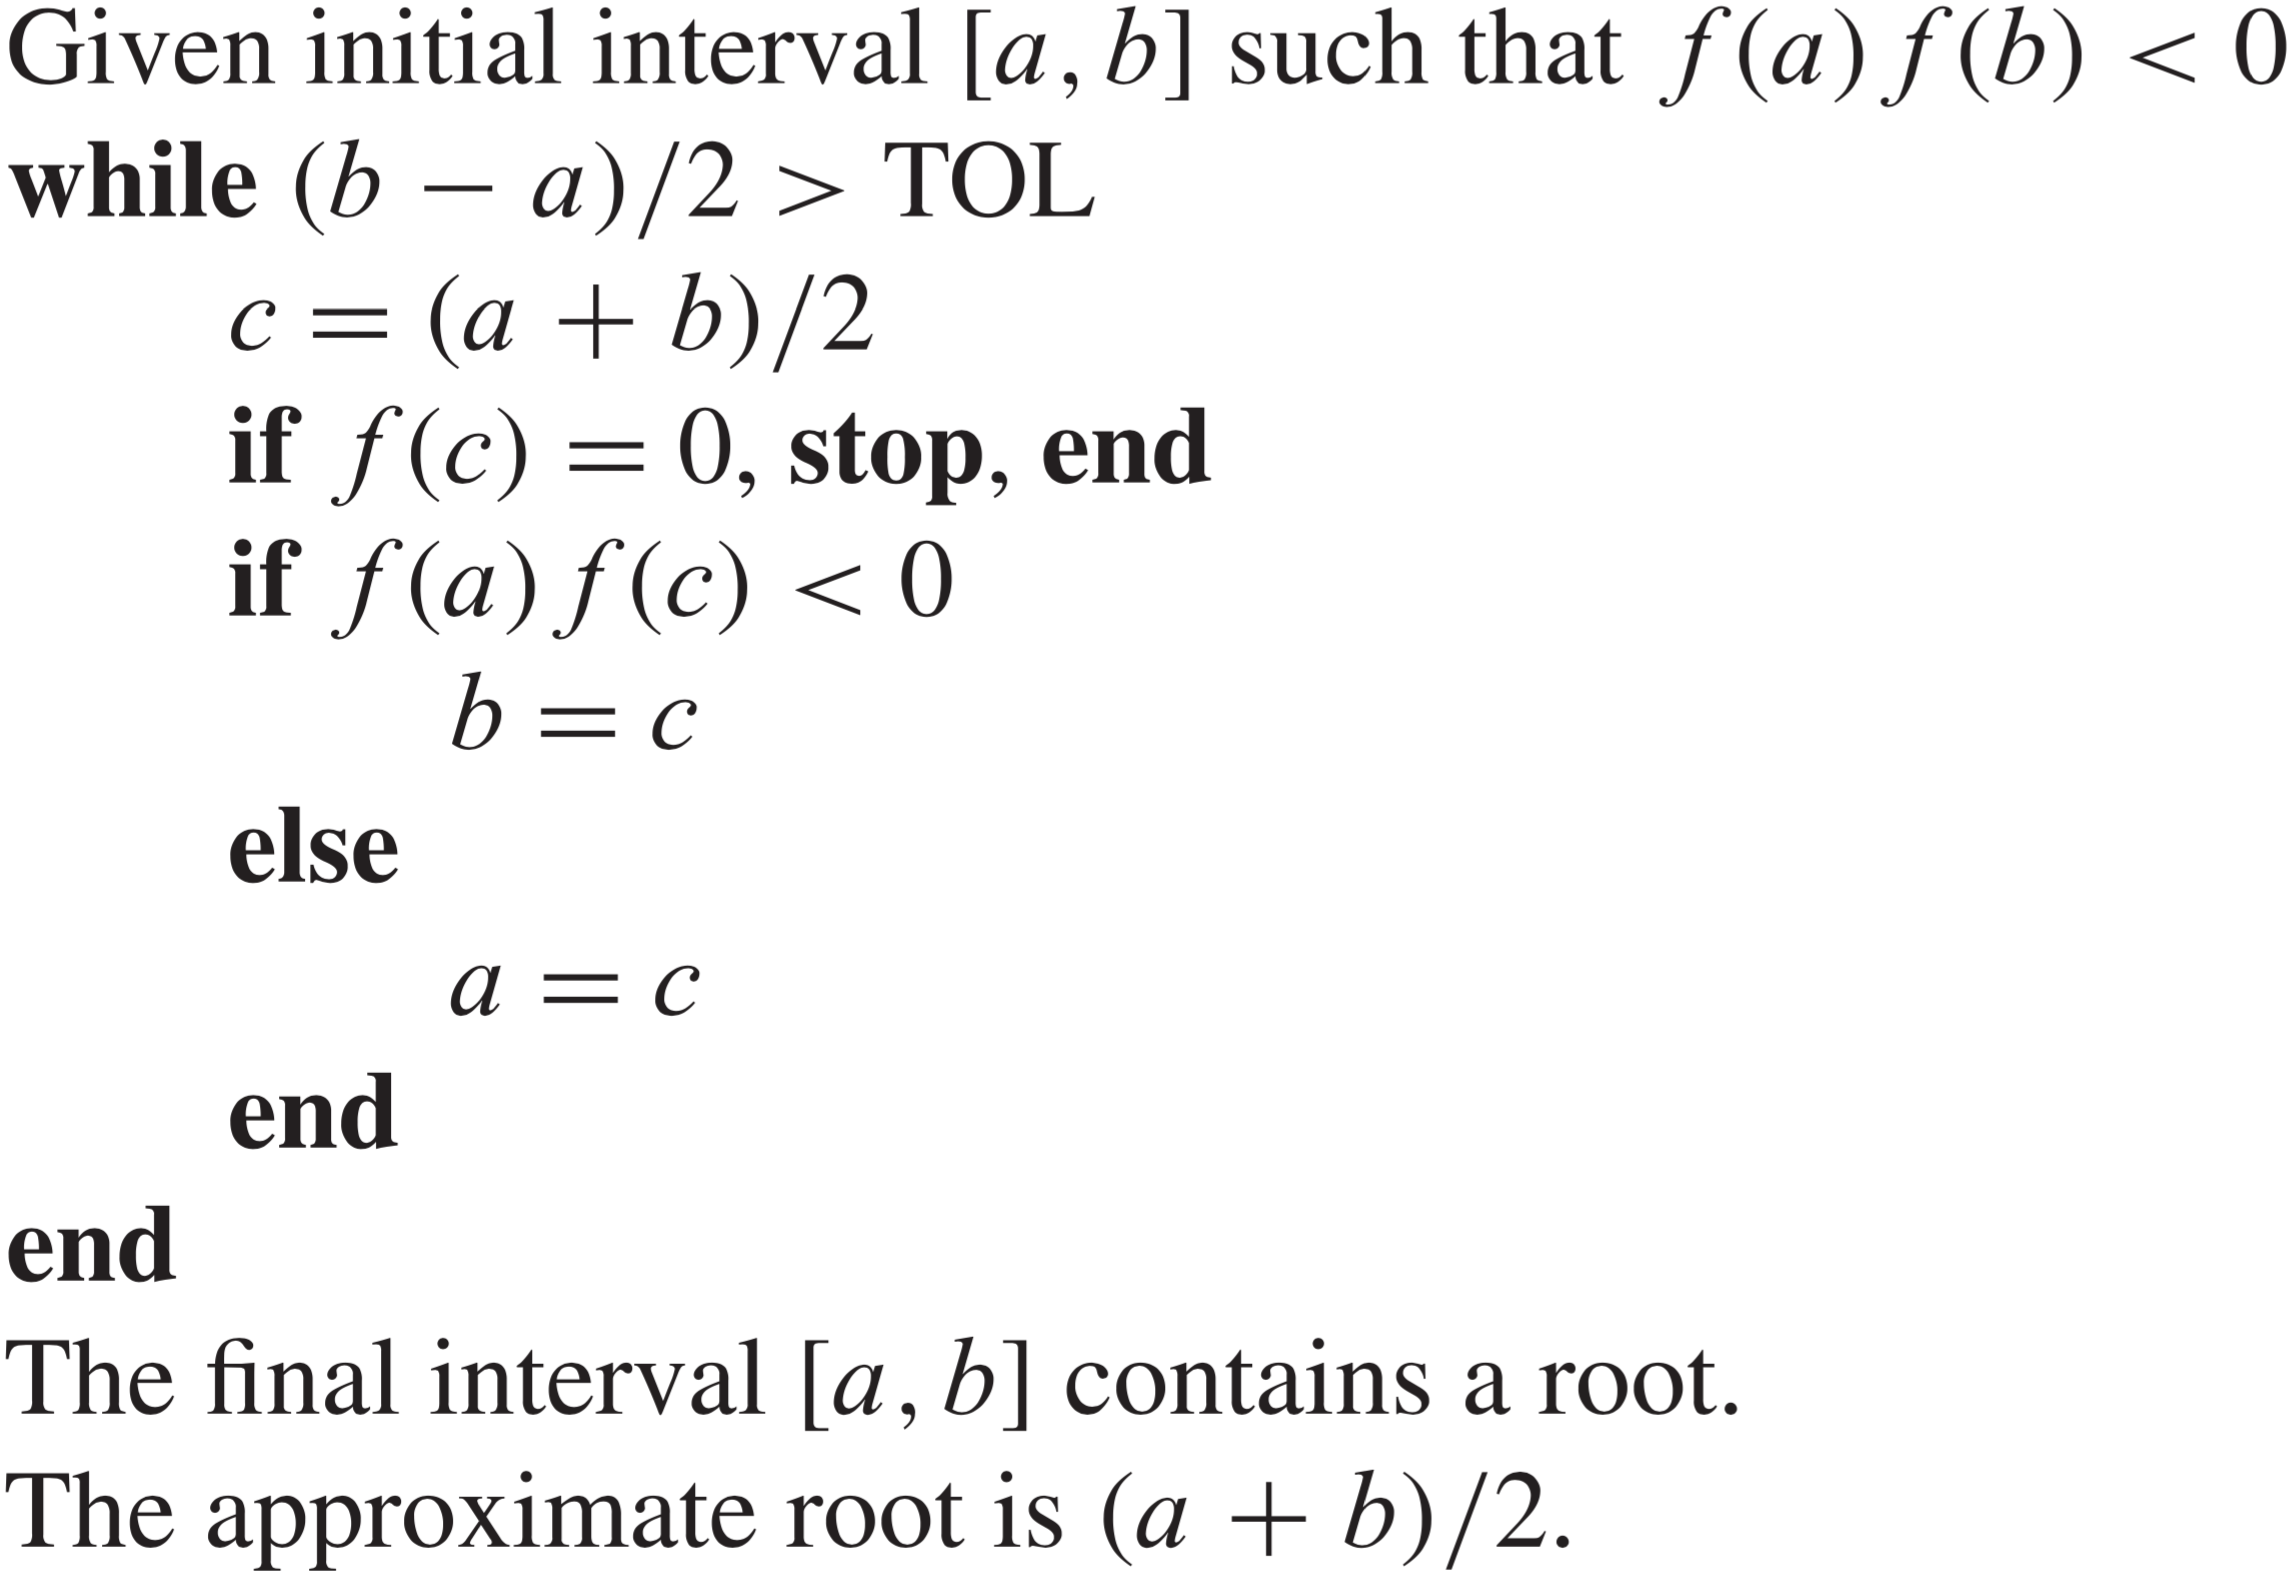
\includegraphics[scale=0.17]{images/bisection_method.png}

% Written pseudocode in MatLab pseudosyntax, men used the book instead (see above)
% \begin{lstlisting}
% %Given initial interval [a,b] such that f(a)f(b)<0
% while (b-a)/2 < TOL
%     c = (a + b)/2;
    
%     if f(c) == 0
%         %End
%     if f(a)*f(c) < 0
%         b = c;
%     else
%         a = c;
% end
% % The final interval [a,b] contains a root
% % The approximate root is (a + b)/2
% \end{lstlisting}

\begin{gather*}
\text{Solution error} = |x_c - r| < \frac{b-a}{2^{n+1}} \\
\text{Function evaluations} = n + 2
\end{gather*}
\subsubsection{Fixed point iteration}
\begin{gather*}
x_0 = \text{initial guess} \\
x_{i+1} = g(x_i) \textbf{ for } i = 0,1,2,... \\
\end{gather*}

\begin{lstlisting}
%Function handle g
% Starting guess x0
% Number of iteration steps k
function xc = fpi(g, x0, k)
x(1) = x0;

for i = 1:k
    x(i+1) = g(x(i));
end

xc = x(k+1);
\end{lstlisting}

\begin{theorem*}
Assume that $g$ is continously differentiable, that $g(r) = r$, and that $S = |f'(r)| < 1$. The Fixed-Point Iteration converges linearly with the rate $S$ to the fixed point $r$ for initial guesses sufficiently close to $r$.
\end{theorem*}

\subsubsection{Newton's method} 
\begin{gather*}
x_0 = \text{initial guess} \\
x_{i+1} = x_i - \frac{f(x_i)}{f'(x_i)} \text{ \textbf{for} i = 0,1,2,...}
\end{gather*}

\begin{theorem*}
Let $f$ be twice continuously differentiable and $f(r) = 0$. If $f'(r) \neq 0$, then Newton's method is locally and quadratically convergent to $r$. The error $e_i$ at step $i$ satisfies
$$
\lim_{i \to \infty} \frac{e_{i+1}}{e_{i}^2} = M,
$$
where
$$
M = \frac{f''(r)}{2f'(r)}.
$$
\end{theorem*}

\begin{theorem*}
Assume that the $(m+1)$-times continously differentiable function $f$ on $[a,b]$ has a multiplicity $m$ at root $r$. Then Newton's Method is locally convergent to $r$, and the error $e_i$ at step $i$ satisfies
$$
\lim_{i \to \infty} \frac{e_{i+1}}{e_{i}} = S
$$
%where $S = {m-1}{m}$
\end{theorem*}

\begin{theorem*}
If $f$ is $(m+1)$-times continuously differentiable on $[a,b]$, which contains a root $r$ of multiplicity $m > 1$, the the \textbf{Modified Newton's Method}
$$
x_{i+1} = x_i - \frac{m f(x_i)}{f'(x_i)}
$$
converges locally and quadratically to $r$.
\end{theorem*}
\hfill 